\section{Materiales y métodos}
\subsection{Carga de datos}
Para poder hacer uso de los datos que se anexan al artículo científico en el que está basado el proyecto, se han de descargar desde la página web del NCBI, con un archivo llamado \textit{setup.sh}. Por otro lado, hay un archivo llamado \textit{launch.sh} que se encarga de ejecutar todos los archivos de R. Se obtienen un total de 21797 genes con 79 muestras cada uno con los que se empieza el análisis.

\subsection{Análisis inicial}
Se crea el archivo llamado \textit{Análisis\_EG\_dataInput.R}, el cual carga los datos y se crea la limpieza y preprocesamiento de los datos. En primer lugar se crea una configuración del entorno de R y se procesan los datos. Se hace uso de la librería de \textit{WCGNA} obtenida desde \textit{Bioconductor}. 

Por otro lado se hace un reajuste de datos, se transforman para que sean las filas las correspondientes a los genes y, las columnas, a las muestras de los mismos.

Como se desconoce si hay alguna falta de datos, se comprueba si hay algún dato que falta o que es nulo. En el caso de que si haya datos no válidos, se eliminan los genes y las muestras de estos.

Luego, se agrupan para poder ver si hay o no valores atípicos y luego se eliminan aquellos que si que lo sean con un corte de altura. 

Todos los datos mencionados anteriormente se almacenan para poder hacer así el análisis de red.

\begin{figure}[!]
	\fbox{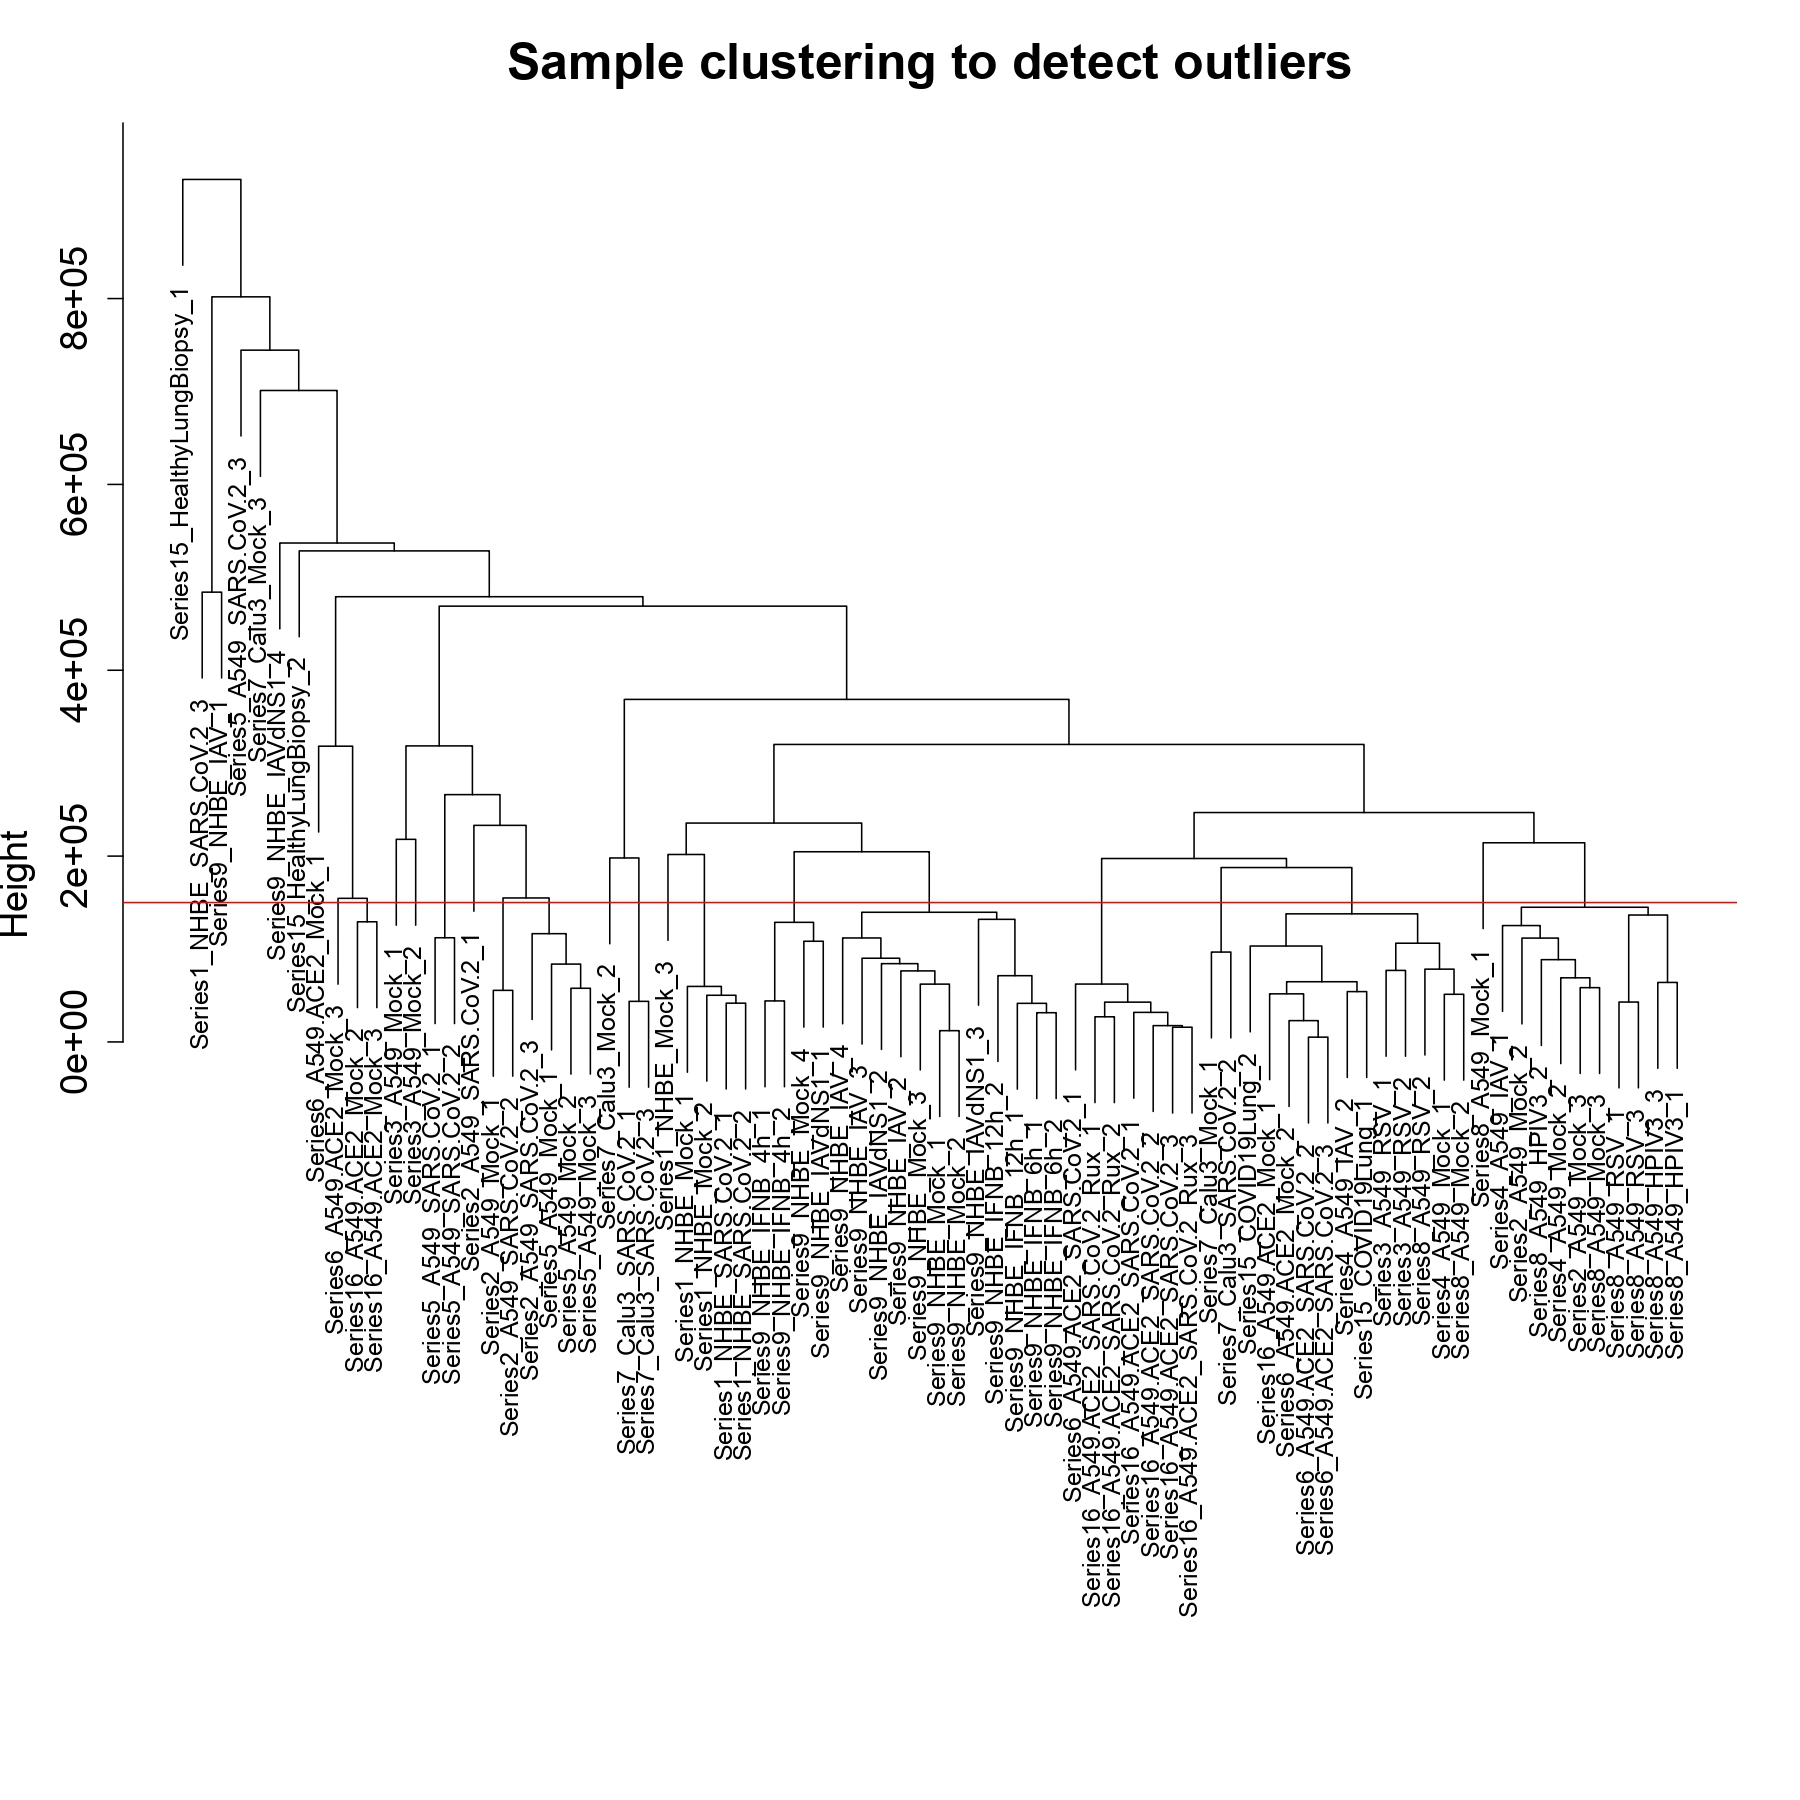
\includegraphics[width=0.9\textwidth]{figures/sampleClustering.jpg}}
	\caption{Sample Clustering}
	\label{fig:sample_clustering}
\end{figure}

